\section{Programación Lógica}

\begin{itemize}
\item Declarativo
\item Basado en lógica formal
\item Se describe el dominio en términos de hechos y reglas de inferencia. Si sucede algo, entonces podemos derivar que sucede otra cosa.
\item El sistema responde a consultas que preguntan por algún hecho.
\item No es un paradigma que se preste a performance, sino a expresividad.
\item Como ejemplo tenemos a Prolog
\item El objeto principal es el predicado. Por ejemplo: cliente(Id,Nombre,Apellido,Email)
\item Esta cercano al modelo conceptual de base de datos.
\end{itemize}


\subsection*{Modelo de ejecución}

\begin{itemize}
\item Nos queda un sistema de ecuaciones al armar el programa.
\item Se utiliza backtracking para ir analizando las soluciones.
\item ¿Que pasa si hay más soluciones? La decisión inicial de probar la primer clausula limito cuanto se ve del árbol de posibles soluciones.
\end{itemize}

\begin{figure}[!htb]
    \centering
    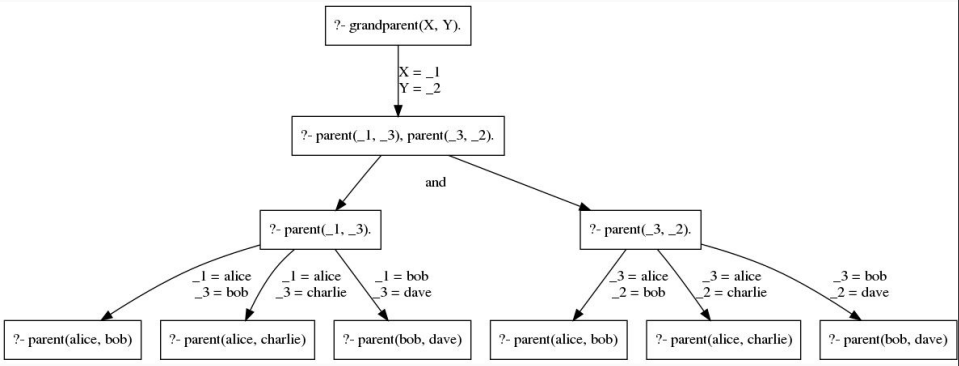
\includegraphics[width=0.7\textwidth]{img/arbolBackTrackingProlog.PNG}
    \caption{X e Y son variables, se realiza una consulta que busca probar si hay algún X e Y de forma tal de que X sea el abuelo de Y. Se prueban las combinaciones de hechos que se tienen en la base de datos para llegar a la solución (true o false)}
\end{figure}


\subsection*{Efectos colaterales}
\begin{itemize}
\item Existen predicados que causan efectos colaterales al cumplirse (por ejemplo un print). Es difícil razonar como interactúan con backtracking
\item Tratar de no usar funciones que dejen efectos colaterales porque pasan cosas impredecibles.
\item Otra opción de efecto colateral seria realizar un corte del árbol, nos puede sacar soluciones que nos podían interesar.
\end{itemize}

